% This is samplepaper.tex, a sample chapter demonstrating the
% LLNCS macro package for Springer Computer Science proceedings;
% Version 2.20 of 2017/10/04
%
\documentclass[runningheads]{llncs}
%
\usepackage{graphicx}
\usepackage{hyperref}

% Used for displaying a sample figure. If possible, figure files should
% be included in EPS format.
%
% If you use the hyperref package, please uncomment the following line
% to display URLs in blue roman font according to Springer's eBook style:
% \renewcommand\UrlFont{\color{blue}\rmfamily}

\begin{document}
\newcommand{\ywa}[1]{\textsf{#1}}

%
\title{Towards More Transparent, Reproducible, and Reusable Data Cleaning with OpenRefine\thanks{Work supported in part by the National Science Foundation, award OAC \#1541450.}}
%
\titlerunning{Transparent, Reproducible, and Reusable Data Cleaning with OpenRefine}
% If the paper title is too long for the running head, you can set
% an abbreviated paper title here
%
% \author{\relax}
\author{Lan Li\inst{1} \and
Bertram Lud\"ascher\inst{1} \and
Qian Zhang\inst{2} 
}
%
%\authorrunning{F. Author et al.}
% First names are abbreviated in the running head.
% If there are more than two authors, 'et al.' is used.
%
% \institute{\relax}
\institute{School of Information Sciences, University of Illinois at Urbana-Champaign, USA 
\email{\{lanl2,ludaesch\}@illinois.edu}
\and
University of Waterloo, 200 University Ave W, Waterloo ON N2L 3G1, Canada
\email{q394zhan@uwaterloo.ca}\\
}

\maketitle              % typeset the header of the contribution

\begin{abstract}
  We study provenance features of OpenRefine, a popular data cleaning tool. In OpenRefine,
  provenance is available through \emph{operation histories} and \emph{recipes}. The former provide
  users with an undo/redo capability; the latter represent histories in JSON, so recipes can be
  reused. The model implicit in histories and recipes exhibits both \emph{prospective} and
  \emph{retrospective} provenance features, but is incomplete in at least two ways: (i) functions
  resulting in mass edits, and (ii) single cell edits are not captured, thus missing important
  prospective and retrospective provenance information, respectively. We propose to complete the
  missing information by capturing names and parameters of user-invoked functions, and by exposing
  retrospective provenance hidden in internal project files. The feasibility of the approach is
  demonstrated with an early prototype.  \keywords{OpenRefine \and data cleaning \and provenance \and transparency \and reproducibility \and reusability} \end{abstract}

\section{Introduction}

OpenRefine \cite{OpenRefine} is a popular data cleaning tool that lets users explore, profile, and
edit datasets in a browser-based, spreadsheet-like GUI. In particular, users can execute various
transformations on columns, e.g., trimming whitespaces, changing case, converting formats and data
types, etc. To create canonical names or values in the presence of variant spellings and
representations, OpenRefine employs powerful clustering methods (\emph{key collision} and
\emph{nearest neighbor}), parameterized by \emph{keying} or \emph{distance functions}. 

Consider an output dataset $D' = W(D)$ resulting from the application of a user-defined data
cleaning workflow $W$ on an input dataset $D$ (often a CSV file). The goal of $W$ is that the output
$D'$ has better \emph{data quality} (is ``cleaner'') than the input $D$ and that $D'$ is ``fit for
use'' \cite{wang1996accuracy,sadiq2013handbook}.

While working on a data cleaning project, a user's linear \emph{operation history} $H$ provides a high-level, human-readable overview of the sequence of steps performed and can be used to undo and redo operations. In addition, the user can extract all or parts of the operation history to obtain a \emph{recipe} $R$ in machine-readable JSON format. This JSON recipe $R$ can then be \emph{reused} on datasets similar to $D$. The history $H$ and its companion recipe $R$ thus provide valuable \emph{provenance} information about $W$. The following are important requirements or desiderata for workflows and provenance artifacts: 

\begin{itemize}
\item  \emph{Transparency.} A skeptical data cleaning customer should be able to explain how $D'$ was obtained from $D$, i.e., what operations were performed on what parts of $D$ and in what order. This is the classical domain of provenance.
\item \emph{Reproducibility.} Given $D$ and a description of $W$,  a skeptic should be able to devise their own implementation $I_W$ such that $I_W(D)$ also yields $D'$.
\item 
\emph{Reusability.} It should be ``easy'' to apply $I_W$ to other datasets $E$ that are ``similar
enough'' to $D$ to obtain a ``cleaner'' $E'$. This notion is necessarily vague, given that
the underlying notions have to be prescribed first. 
\end{itemize}

\begin{figure}[t]
\centering
%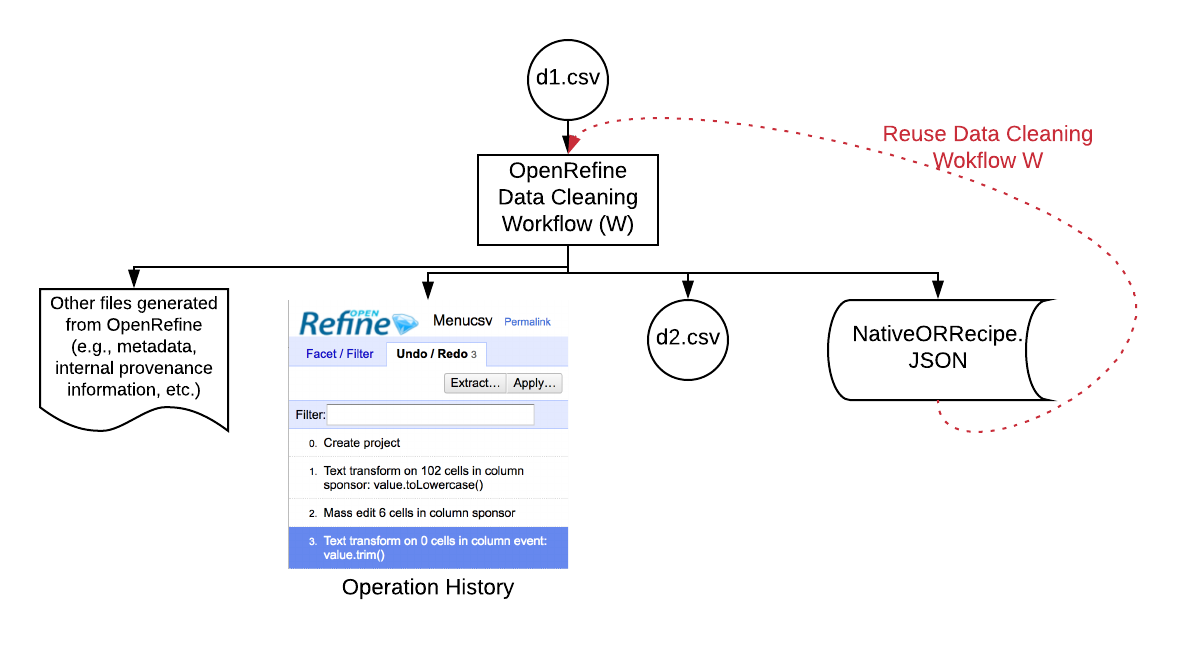
\includegraphics[width=100mm,scale=0.7]{figs/DC.png}
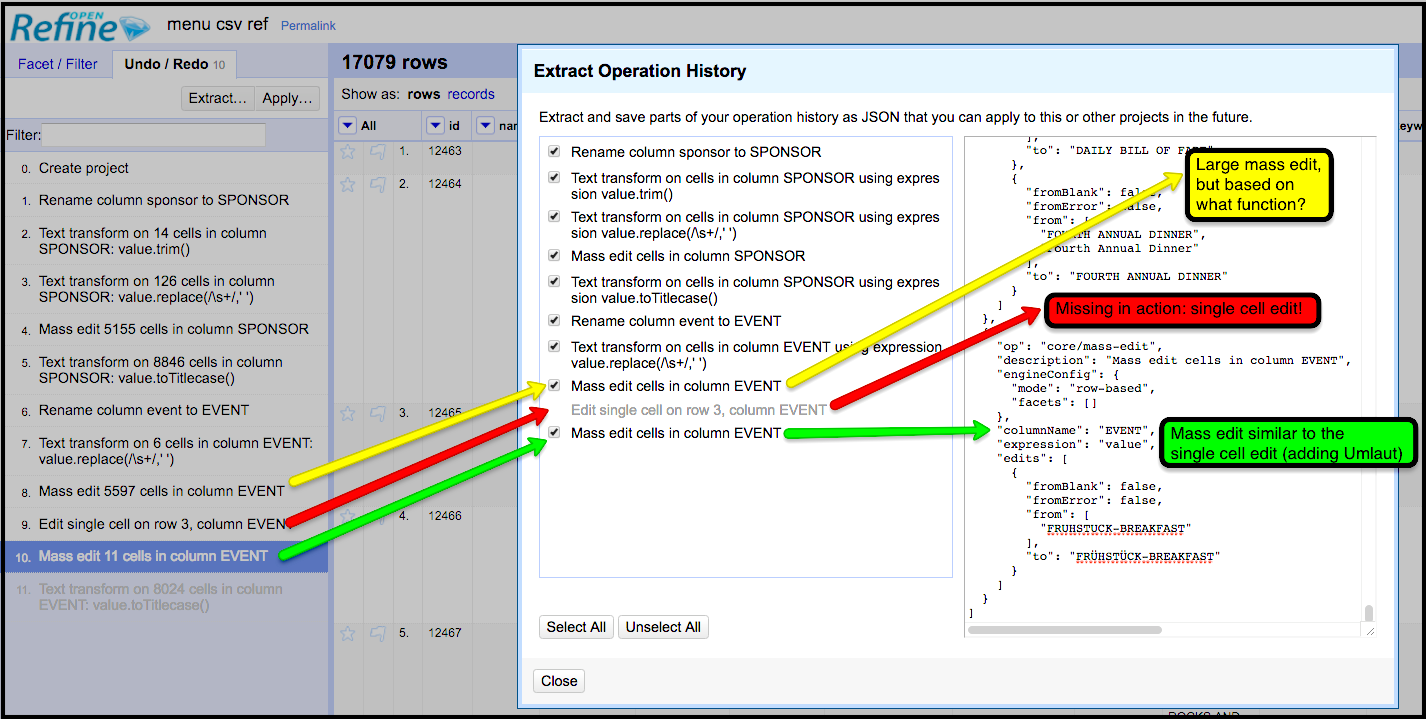
\includegraphics[width=0.95\textwidth]{figs/OR-missing-brighter.png} 
\caption{From Steps 1--10  of the history $H$ (background, left) the user can extract a machine-readable JSON recipe $R$ (bright foreground, right). The \emph{mass edit} in Step 8 is captured via a set of rules $\{$\texttt{from}:\emph{old} $\to$ \texttt{to}:\emph{new}$\}$, but it is \emph{not} recorded which function was used to create these rules. The \emph{single cell edit} in Step 9 is greyed out and cannot be selected by the user for inclusion in  $R$. Neither $H$ nor  $R$ indicate what this edit was. In contrast, the mass edit in Step 10 is included in the recipe $R$: it is fully described by the rule \texttt{from:FRUHSTUCK-BREAKFAST} $\to$ \texttt{FR\"UHST\"UCK-BREAKFAST} that has been (and can be, prospectively)  applied  to all values in the EVENT column.
}  
\label{fig:missing} 
\end{figure}



\section{Provenance and OpenRefine}\label{sec:prov-openr}

We distinguish \emph{prospective provenance} which is the specification of a workflow $W$ or at
least of $W$'s dataflow dependencies, and \emph{retrospective provenance} which records runtime
observables used to instantiate $W$. In OpenRefine the user workflow $W$ is partially captured in
the operation history $H$ and the associated recipe~$R$, which can thus serve as an implementation
$I_W$. However, as illustrated in Figure~\ref{fig:missing}, $R$ is \emph{incomplete}: If the user
chose a \emph{Cluster \& Edit} method, e.g., \emph{key collision} with $n$-gram \emph{fingerprint}
function for $n=3$, then $R$ only captures rules $\{$\texttt{from}:\emph{old} $\to$
\texttt{to}:\emph{new}$\}$, but not the method, function, or parameters. Thus prospective provenance
is lost and reusability diminished. If the user performs a \emph{single cell edit}, say fixing
umlauts in a particular cell, then this ``one-off'' is not considered a reusable operation and
(understandably) omitted from the recipe $R$. However an important piece of retrospective provenance
is lost this way, reducing transparency and preventing reproducibility of $W$ via $R$.


\section{Approach and Demonstration}\label{sec:appr-prot-demonstr}

\begin{figure}[t] 
\centering
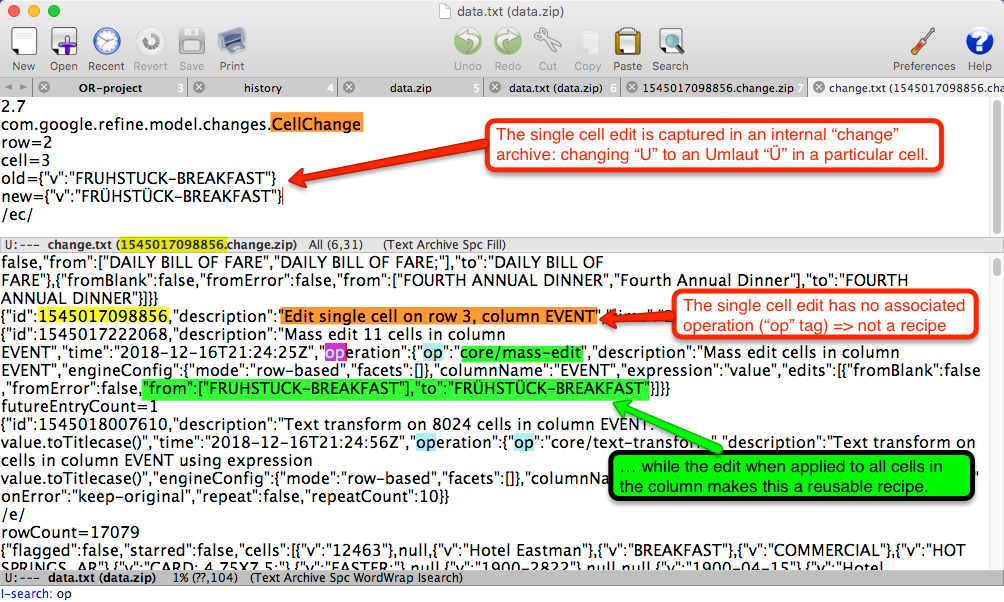
\includegraphics[width=0.95\textwidth]{figs/OR-internal.png}
\caption{OpenRefine project files reveal missing retrospective provenance: the \texttt{data} zip-archive contains a reference to a single-cell edit (center left); the individual update is recorded in a \texttt{change} archive in a history folder (top). } \label{fig-archives}
\end{figure}
 
We propose to enhance the native OpenRefine recipes as follows: when users select operations such as
\emph{Cluster \& Edit}, the system should also capture \emph{prospective} information such as the
clustering method with associated functions and parameters. Missing \emph{retrospective}
information, e.g., from single cell edits should be extracted from internal OpenRefine files and
made explicit (Figure~\ref{fig-archives}).

\begin{figure}[h]
        \centering
        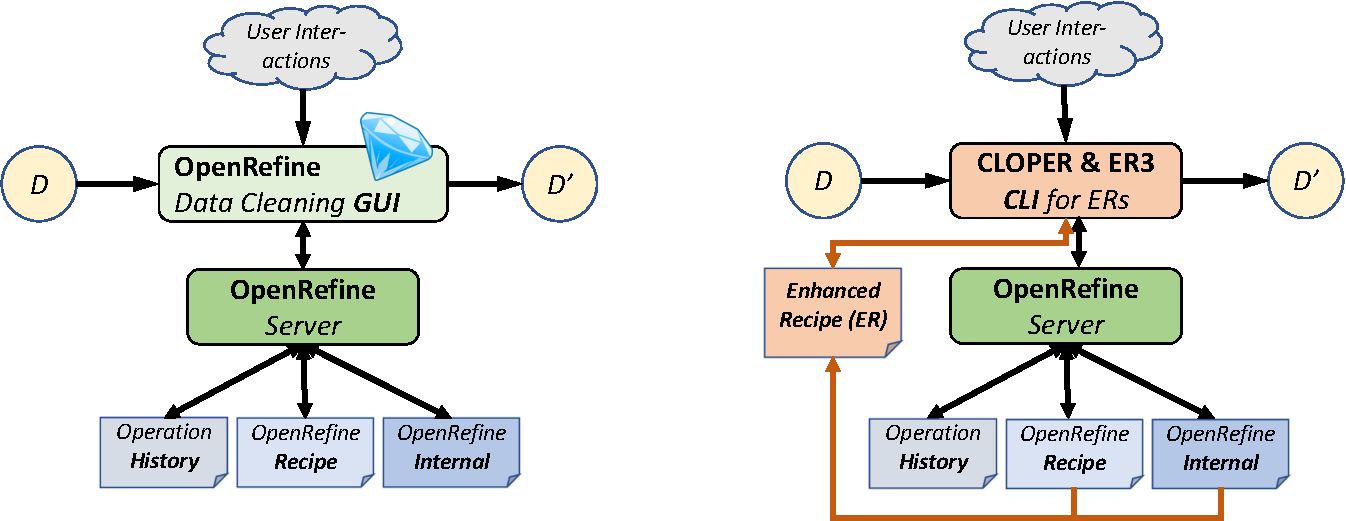
\includegraphics[width=\textwidth]{figs/reproducible-OR-crop} 
        \caption{Driven by user interactions in the OpenRefine (OR) GUI, input dataset $D$ is transformed
          (cleaned)  to obtain $D'$. The OR server captures provenance information in a
          user-readable history $H$, machine-readble JSON recipe $R$, and internal project files.
          CLOPER is used to capture additional provenance in an enhanced recipe (ER). The ER
          Re-Runner (ER3) can execute native recipes and enhanced recipes}\label{fig-CLOPER-ER3}
\end{figure}
 
To demonstrate our approach we have developed CLOPER (Command-Line OpenRefine Prototype for Enhanced
Recipes) and ER3 (Enhanced Recipe Re-Runner) \cite{ORtools2018}, both of which use a Python client
library \cite{makepeace18ORclient} to communicate with the OpenRefine server. CLOPER can execute
OpenRefine operations via a command-line driven interface (i.e., without a GUI) and adds missing
prospective information to recipes (Figure~\ref{fig-CLOPER-ER3}). ER3 can then run those enhanced
recipes and demonstrate the improved transparency, reproducibility, and reusability. Further
extensions to CLOPER and ER3 to add additional prospective and retrospective provenance are under
development.


\bibliographystyle{splncs04}
\bibliography{datacleaning}


% \begin{thebibliography}{8}

% \bibitem{ref_proc1}
% Dey, S., Belhajjame, K., Koop, D., Raul, M.,Lud\"ascher, B.:Linking prospective and retrospective provenance in scripts. In: Theory and Practice of Provenance. In: 9 International Journal of Digital Curation. (2015)

% \bibitem{ref_lncs1}
% Zhao, Y., Wilde, M., Foster, I.:Applying the virtual data provenance model. In: International Provenance and Annotation Workshop pp. 148-161. Springer, Berlin, Heidelberg.(2006, May)

% \bibitem{ref_url1}
% OpenRefine-client Library Github, \url{https://github.com/opencultureconsulting/openrefine-client}. 


% \end{thebibliography}





\end{document}

